\chapter{Concept}
In this chapter a concept including intraoperative 3D reconstruction of the liver and
intaoperative resection planning will be presented. 

% Typical concept: \cite{payan2012soft}
\section{Overview}
The desired concept differs in some places from conventional approaches, but not
everything changes (Figure \ref{fig:ConceptChanges}). Conventional approaches
plan the surgery based on the preoperative CT data very accurately on a 
3D model of the liver. Then at the
beginning of
the surgery, because the liver has probably changed its shape since preoperative
scanning, the whole preoperative model (including the preoperative planning) must be deformed again 
intraoperatively \cite{payan2012soft}.

The new approach is to create a 3D model of the liver during
the surgery and plan based on this model. This means that a registration does
not have to be done anymore. The created model will not be a complete
model of the liver but it will be an undeformed one. Actually, such
intraoperative models are already created with conventional approaches, they are only used for registration
and not for navigation. Before the planning also the tumor has to be
reconstructed intraoperatively.

The hardware for this concept consist of an optical tracking camera (Polaris, NDI, Canada), a tracked
intraoperative ultrasound (Flex focus 800, BK Medical, Denmark) and a computer with a 2D and a 3D monitor (CAS-One Navigation platform, CAScination AG,
 Switzerland) (Figure \ref{fig:HWcolored}). The
tracking camera is used to track the ultrasound and other surgical tools used
during the intervention. The ultrasound is used to reconstruct the 3D model of
the liver with its tumors and the computer with the monitors is used to
visualize the 3D model and planning of the resection. The 2D monitor has a touch
interface such that the surgeon can interact with the software.

In order to be able to perform an intervention with this new approach, new
functionalities must be developed.
\begin{figure}[H]
  \centering
  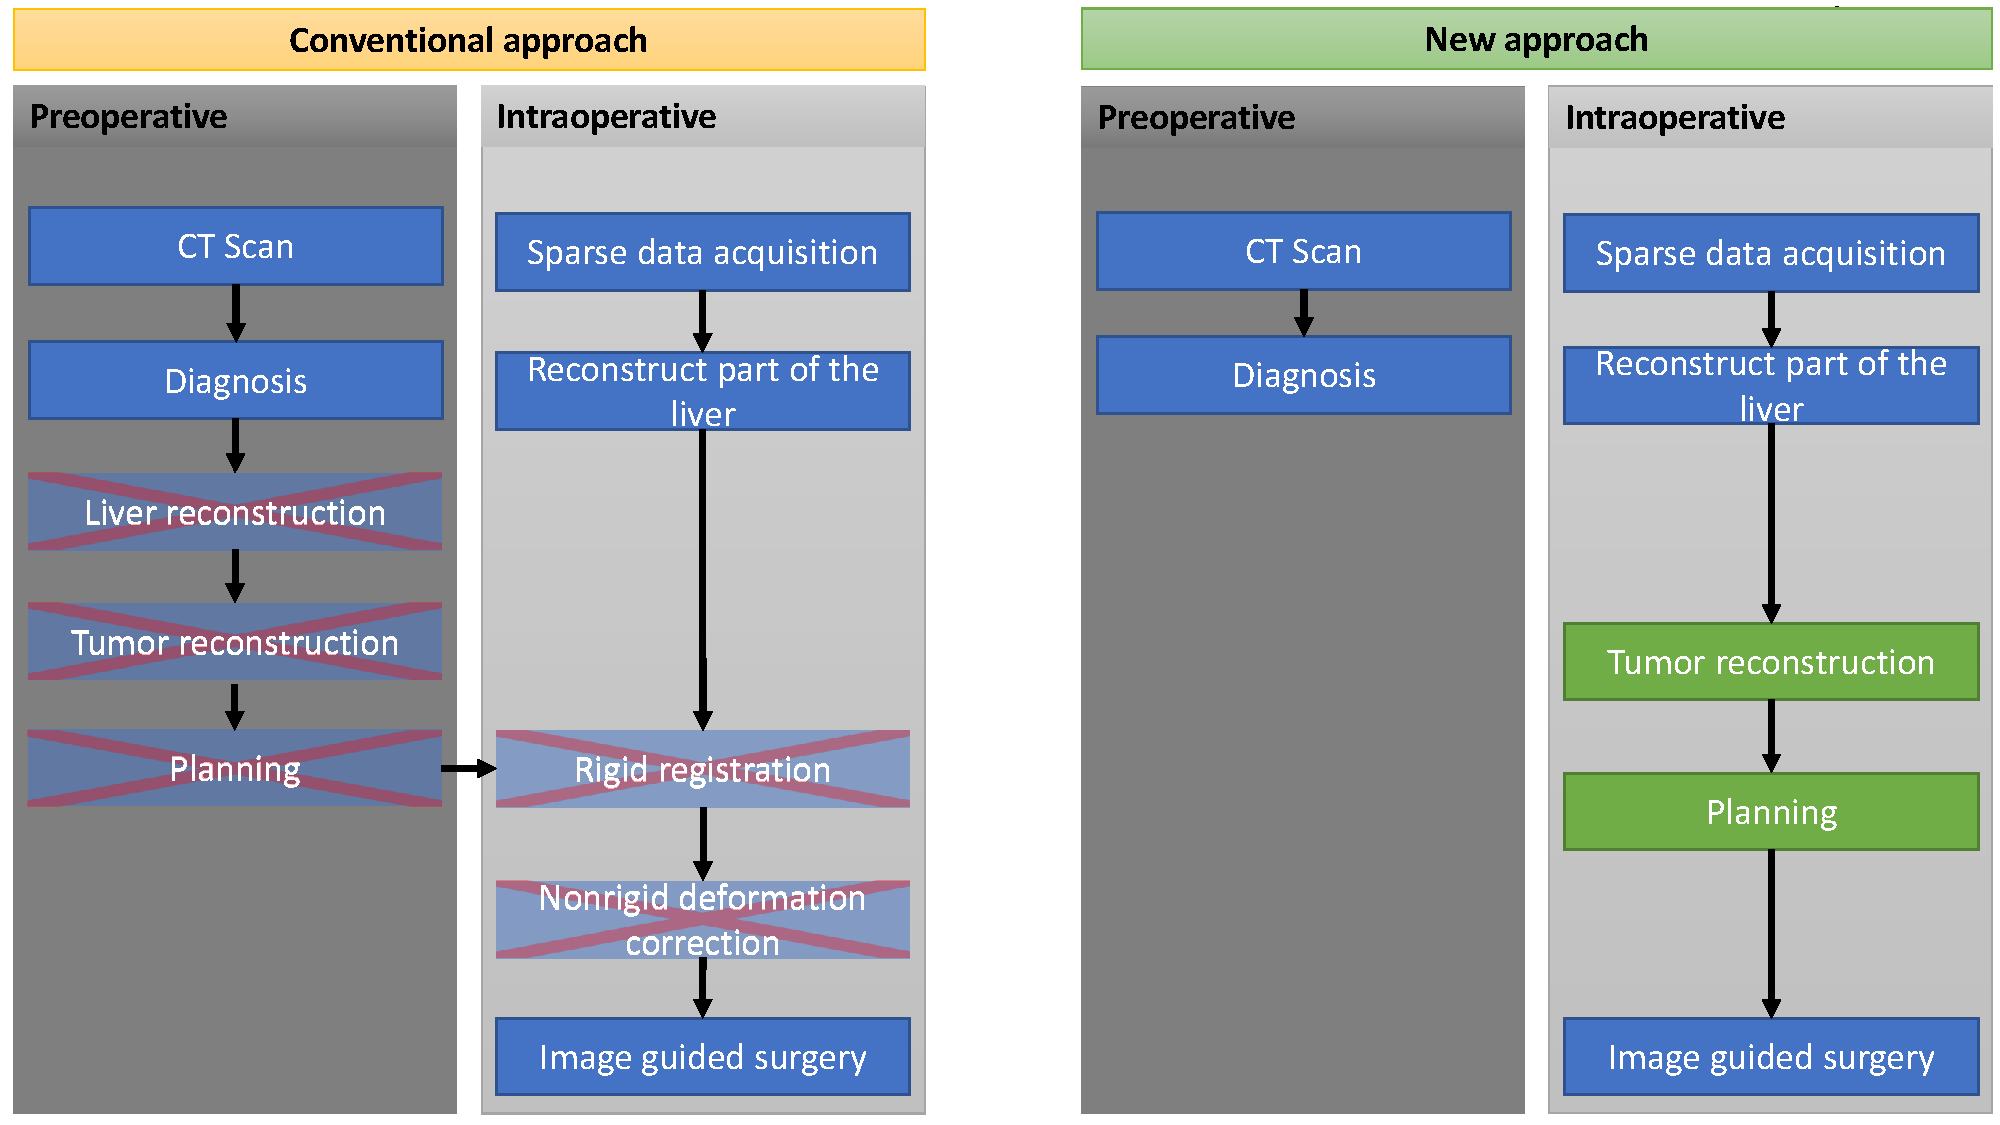
\includegraphics[width=1.0\textwidth]{ConceptChanges}
  \caption{The changes from a conventionally navigated liver surgery procedure to the
    proposed new way of navigating during a liver resection surgery. In the dark gray boxes are the things
  that are done preoperatively and in the bright gray boxes the things that are
  done intraoperatively. Boxes with
    a red cross will not be need with the new approach and green boxes are not
    needed with the conventional approach.}
  \label{fig:ConceptChanges}
\end{figure}
\begin{figure}[H]
  \centering
  \includegraphics[width=0.6\textwidth]{HWcolored}
  \caption{The setup in the operating room: Red the surgeon; Yellow the
    tracking camera; Green the ultrasound probe; Dark blue the 3D screen; Light
    blue the 2D screen.}
  \label{fig:HWcolored}
\end{figure}

% The hardware used with this system consists of:
% \begin{itemize}
%   \item a tracked ultrasound device
%   \item a tracked pointer tool
%   \item an optical tracking camera to track the instruments
%   \item a computer to run the software
%   \item a 3D-monitor which displays the 3D contents of the software 
%   \item a touch-screen on a 2D-monitor to operate the software and show the
%     ultrasound images
% \end{itemize}
% The software in this system consists of:
% \begin{itemize}
%   \item a sampling method 
%   \item a reconstruction method 
%   \item a segmentation method 
%   \item a planning method 
%   \item a navigation 
% \end{itemize}

% \begin{figure}[H]
%   \centering
%   \begin{tabular}[H]{c c c c c c}
%     \multicolumn{2}{c}{\thead{Sampling method \\ to collect points on \\ the liver-surface}} & \multicolumn{2}{c}{\thead{Reconstruction method \\ to reconstruct the surface \\ from the sampled points}} & \multicolumn{2}{c}{\thead{Segmentation method \\ to segment the tumors on \\ the ultrasound images}}
%     \\
%     \multicolumn{2}{c}{\addheight{
\includegraphics[width=0.3\linewidth]{samplingMethod}}} &
%     \multicolumn{2}{c}{\addheight{
\includegraphics[width=0.3\linewidth]{reconstructionMethod}}} &
%     \multicolumn{2}{c}{\addheight{
\includegraphics[width=0.3\linewidth]{segmentationMethod}}} 
%     \\
%     \\
%     \\
%     \multicolumn{3}{c}{\thead{Planning method \\ to plan the resection \\ of the liver}} & \multicolumn{3}{c}{\thead{Navigation mode used \\ to navigate during the \\ removal of the tumor}} 
%     \\
%     \multicolumn{3}{c}{\centering \addheight{
\includegraphics[width=0.48\linewidth]{planningMethod}}} &
%     \multicolumn{3}{c}{\addheight{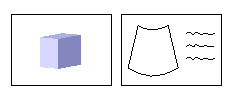
\includegraphics[width=0.48\linewidth]{navigationMode}}} 
%     \\
%     & & & & &
%     % \addheight{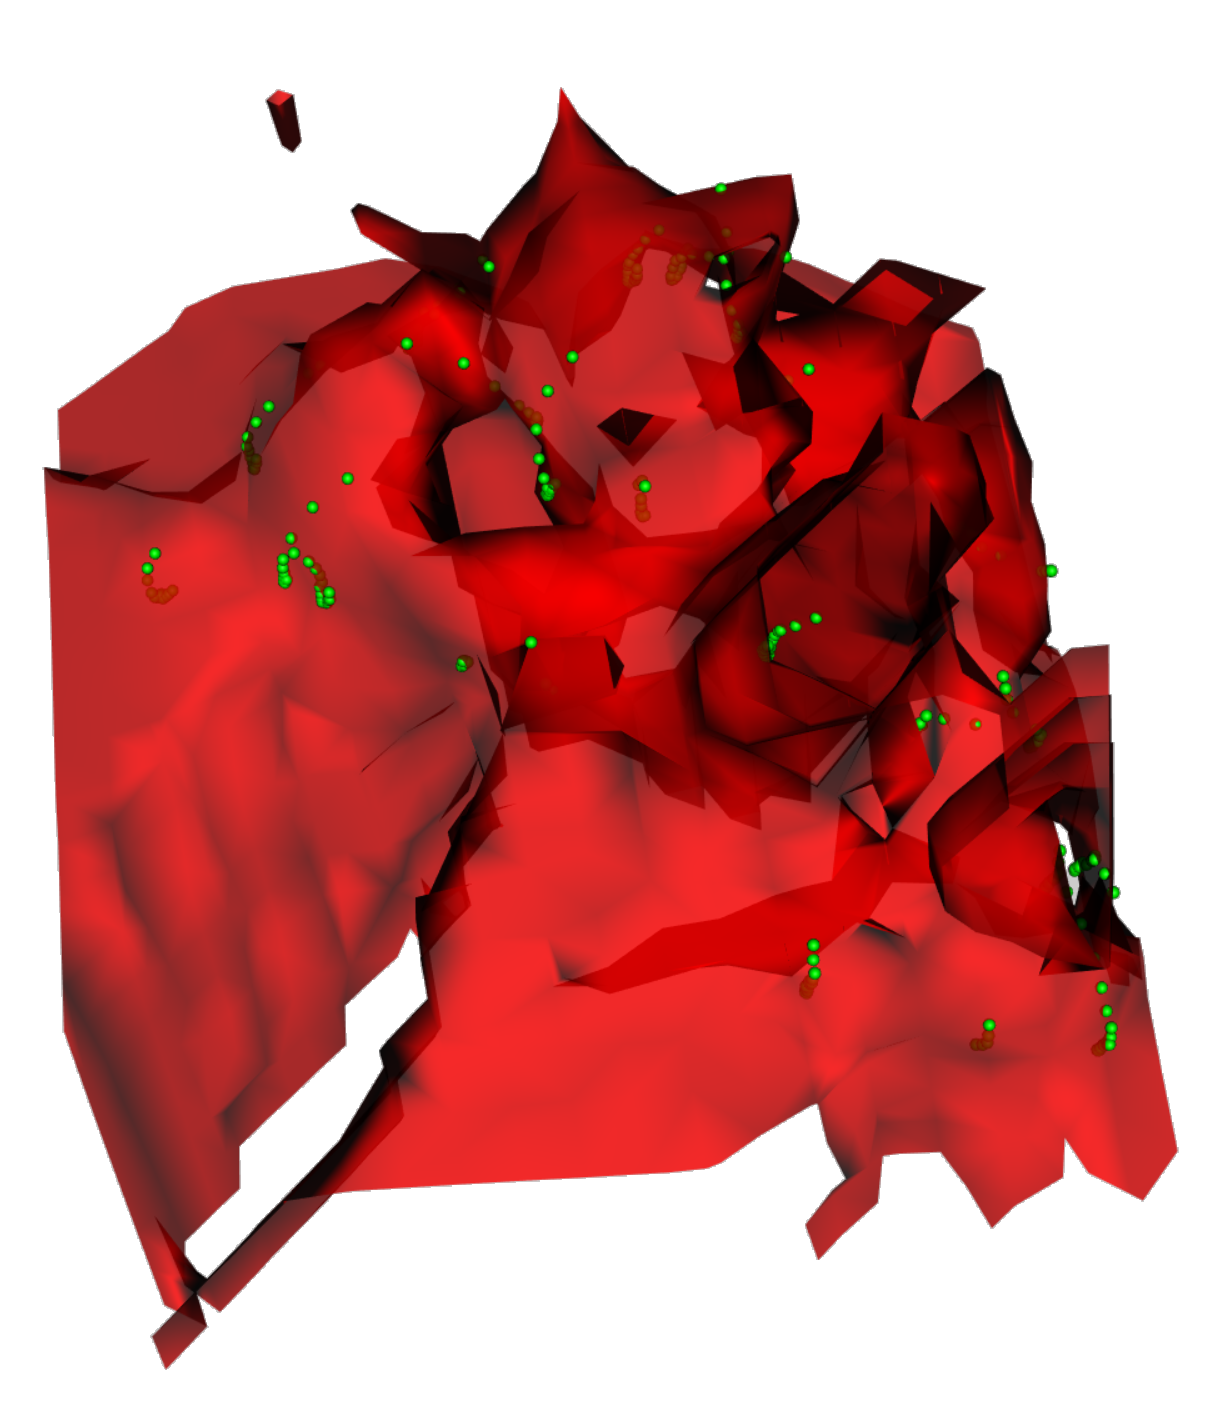
\includegraphics[width=0.3\linewidth]{mes08_pointgrid.png}}
%     \\
%   \end{tabular}
%   \caption{Software components}
%   \label{fig:softwareComponents}
% \end{figure}
\section{Functionalities}
The three main functionalities of the developed concept will be presented in
this chapter. These functionalities were specifically developed for this project.
\subsection{Surface Reconstruction}
During surgery ultrasound images and their corresponding 6D poses (positions and
orientations) are collected and analyzed. First each ultrasound image has to be
checked for contact with the liver. If the ultrasound passes the check, that
means the ultrasound image looks like an ultrasound image that can only arise
when the ultrasound probe lies on the liver surface, then the position of this
image can be used.

\begin{figure}[H]
  \centering
  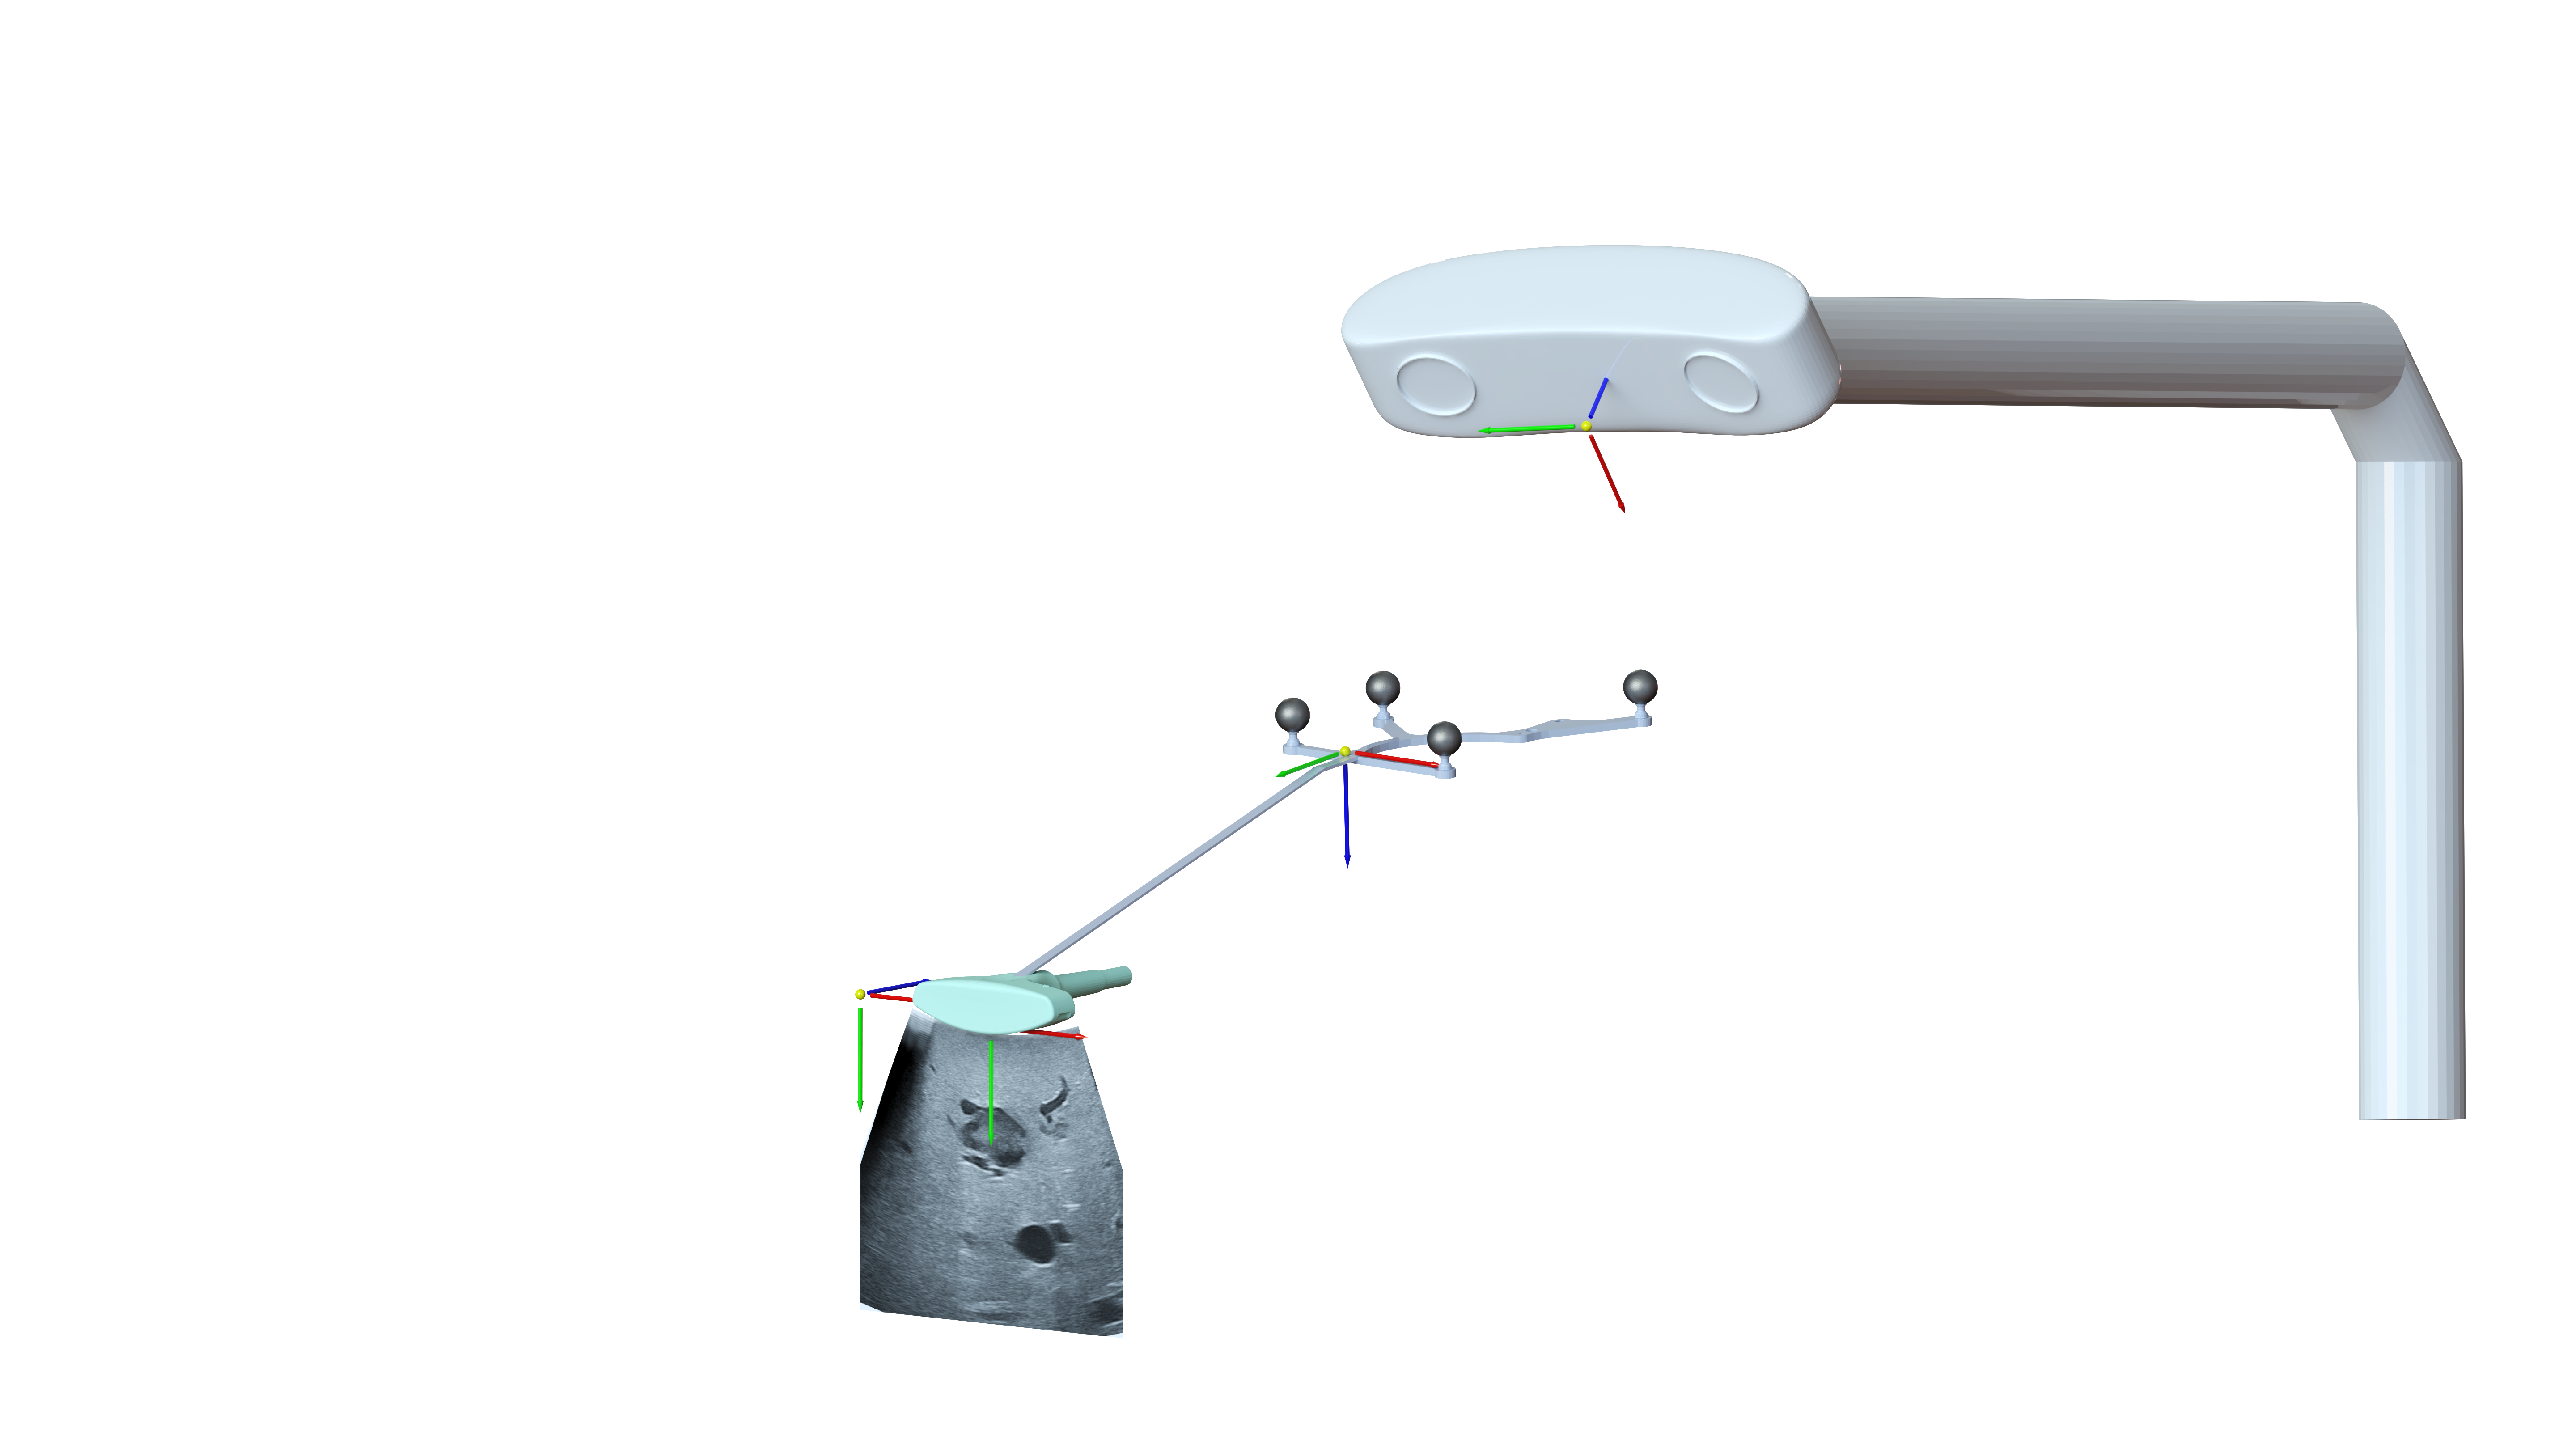
\includegraphics[width=1.0\textwidth]{Render}
  \caption{The different coordinate systems and the transformations between them.}
  \label{fig:Render}
\end{figure}

% \textcolor{green}{In order to use ... too complicated. Put an image for that and name the transformations.}
In order to use the sampled position corresponding to an image, this
position has to be transformed into the correct coordinate system first. There
are four different coordinate systems (Figure \ref{fig:Render}).

The first coordinate system is the image
coordinate system. The units in the \textbf{image coordinate system} are pixels and the
origin is in the top left corner of the ultrasound image.
The second coordinate system is the \textbf{ultrasound coordinate system}. The origin of this
coordinate system is at the probe tip in the middle and the units in this and
the other coordinate systems are millimeters.
The third coordinate system is the
\textbf{marker coordinate system}. The origin is at a user defined
location, relative to the reflective marker spheres.
The final coordinate system is the \textbf{camera coordinate system}. The origin of this
coordinate system is at the position sensor in the tracking camera and can not
be changed.

At the end of this transformation chain, a image pixel 2D position was
transformed into a tracking camera 3D positon and the units changed
from pixel to millimeter. This 3D location in the tracking camera coordinate system
can be added to the collection of points to later reconstruct the surface from.

After collecting the surface points, a reconstruction algorithm reconstructs the surface from these points.
\subsubsection{Surface reconstruction from unorganized points}
% \textcolor{green}{First, collecting the sample ... These terms should match the titles below
% Both other chapters, explain first what the process is for, then what methods are available}
A surface reconstruction's goal is to create a surface from sampled points \cite{berger2017survey}. Two
main steps need to be processed. First, acquisition of the data to create a sample. Secondly,
apply a reconstruction algorithm on the sampled points.

\paragraph{Data acquisition}
% \textcolor{green}{what the process is for, then what methods are available}
In order to reconstruct a surface it is necessary to have some information about
it. Therefore a set of points which lie on or near the unknown surface is acquired first. A
reconstruction algorithm has then to reconstruct the surface from these points.

There exist different methods to collect surface points
\cite{franca20053d}\cite{levoy2000digital}\cite{cui20113d}\cite{chu2002infrared}\cite{dou20153d}.
Optical (non-contact scan) scans are the most popular ones. Specialy laser based
scanners can scan very fast and with a precision in the order of micrometers. Also contact scans exist
\cite{pai2001scanning}. Contact scans can also be very precise (in the order of
micrometers).

In the field of liver surface scanning only a few articles were published  \cite{maier2014comparative} \cite{thompson2015accuracy}. 
They used stereo laparoscopic cameras to sample the surface.

\paragraph{Reconstruction algorithms}
% \textcolor{green}{ switch explicit and implicit, so you have the same order as in the figure}

% \textcolor{green}{what the process is for, then what methods are available}
The problem
surface reconstruction aims to solve is the representation of a surface in 
digital form, from error containing data that has first been scanned in the
real world.

Again, a lot of reconstruction algorithms exist \cite{lim2014surface}, but not
all of them are made to reconstruct from unorganized points. This means
that the point orders, orientations, connections and the topological type of the
surface is not known a priori. Therefore it is necessary that the algorithm does not assume any structure
on the data points \cite{hornung2006robust} \cite{yu1999surface}. The orientations, connections and the topological
type must be inferred from the points. This is a major difficulty of the general surface
reconstruction problem \cite{hoppe1992surface}. In the past few decades, many
algorithms that can solve this problem have been published. Nevertheless it is
still a challanging task that is part of current research \cite{li2018surface}.
The available reconstrction types can be classified into two groups: implicit
volume-based and explicit mesh-based reconstructions (Figure \ref{fig:ImplicitVSExplicit}).
\begin{figure}[H]
  \centering
 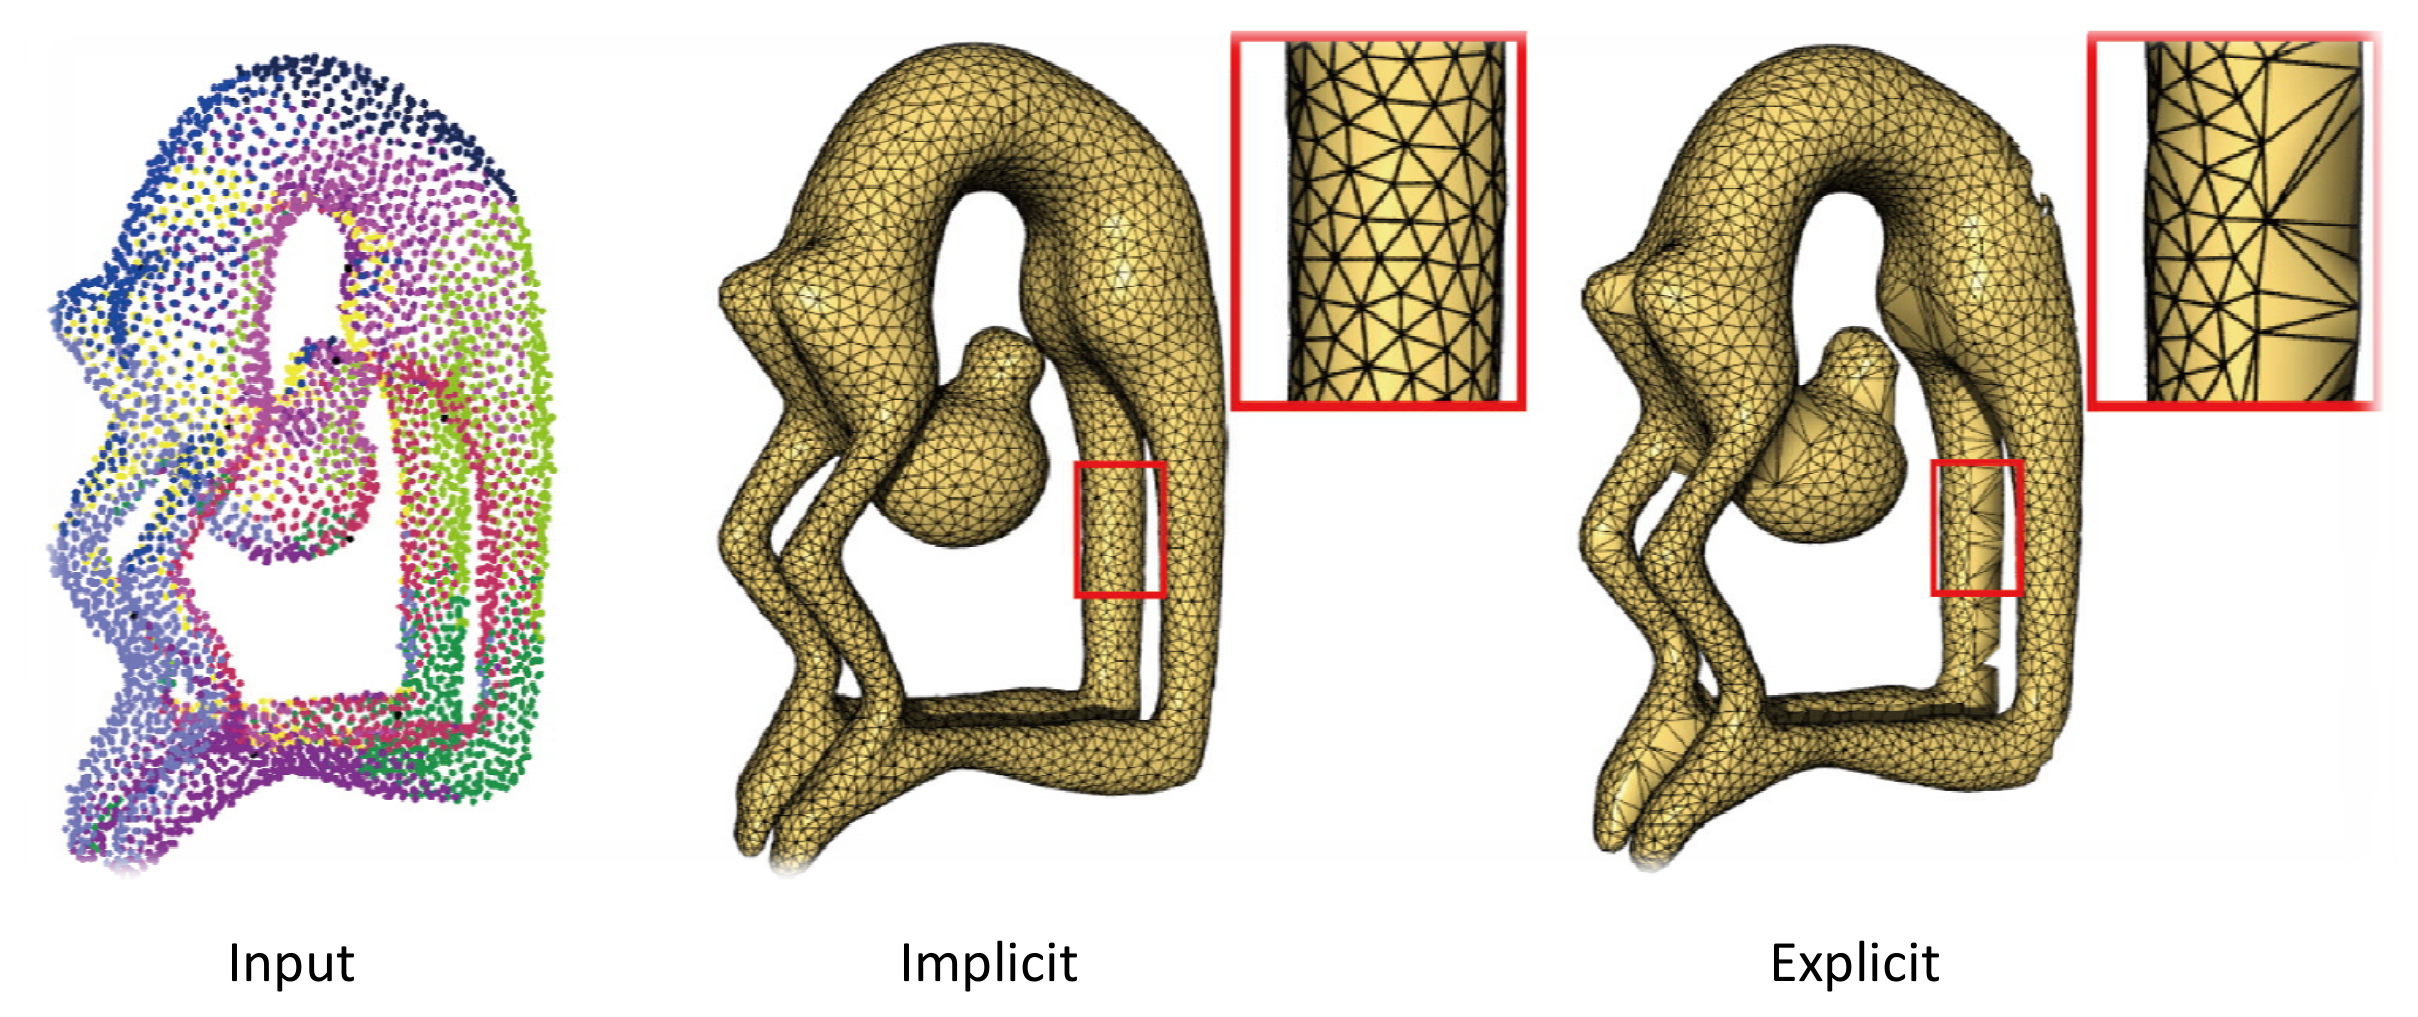
\includegraphics[width=\textwidth]{ImplicitVSExplicit}
 \caption{The difference between implicit and explicit surface reconstructions.
   On the left side is the pointcloud used as input. In the middle the result of an
   implicit reconstruction. On the right side the result of an explicit
   reconstruction \cite{stanfordPP}}
  \label{fig:ImplicitVSExplicit}
\end{figure}
\subparagraph{Implicit volume-based reconstrction}
Implicit volume-based reconstruction techniques construct an implicit
volume-function from the input points. From the iso-surface of the
volume-function a restored surface can then be optained. For these methods it is
not a problem if the surface topology is complex. But most of these methods
suffer from oversmoothing the data and the need of accurate directions of normal
vectors in addition to the unorganized points. 
\subparagraph{Explicit mesh-based reconstrction}
Explicit mesh-based reconstrction methods form a triangular mesh directly from
the unorganized points. These mesh-based reconstructions are precise but they
have problems with noise, complex shapes and especially holes in data (Figure
\ref{fig:ImplicitVSExplicit} right image).
\subsection{Tumor Segmentation}
To reconstruct and later plan the resection of a tumor, the shape
of the tumor has to be made visible first. Because most liver tumors are not visible from the outside of the liver, an
ultrasound device is often used during liver resections to look behind the
liver surface.

Therefore this ultrasound device should also be used to
reconstruct the shape of a tumor. This is done by segmenting the same tumor on
multiple ultrasound images. Depending on the desired resolution of the
reconstructed tumor, more or less images have to be segmented. With the corresponding
poses of the ultrasound images, the 3D positions of the individual contour
pixels can be calculated. These positions will create a point cloud that
represents the shape of the tumor. This shape can then be reconstructed by a
surface reconstruction algorithm.

To make an accurate and fast reconstruction of the tumor possible a fast segmentation of the tumor is
necessary. For this reason, we employed a semi-automatic segmentation algorithm.

\subsubsection{Semi automatic 3D segmentation}
In order to semi automatically segment a tumor in the liver, the segmentation
has to be initialized manually. To do so, a sphere needs to be
placed in the center of the tumor manually. Afterwards each ultrasound image
which cuts this sphere will be segmented automatically with the cut area as
an initialization for the segmentation. These segmentations would be used to
reconstruct the surface of the tumor. An accurate reconstruction of the tumor
surface would enable for optimized resection planning.

\subsection{Resection Planning}
For parenchymal-sparing liver resections, the goal is to keep as much healthy tissue as
possible. When the tumor's location in the liver and the size are known, one can plan a
precise resection from these information. The surgeon is able to choose
which shape the resection plane will have and how much safety margin he wants to
add around the tumor. Then a resection plane which fulfills the desired requirements
will be shown to the surgeon. This resection plane could then be fine tuned before the
surgeon starts the resection.
% After collecting the needed
% information as described in the previous sections, the planning can 

\section{Workflow}
In this section the conceptual workfolw for a liver resection using the
desired system will be presented. The following flow diagram shows the five main
steps (Figure \ref{fig:conceptWorkflow}).
\begin{figure}[H]
  \centering
  \smartdiagram[sequence diagram]{Preparation, Liver scanning, Tumor scanning,
    Resection planning,  Removal of the tumor}
  \caption{The main steps the surgeon has to do during a surgery with the
    proposed system.}
  \label{fig:conceptWorkflow}
\end{figure}
In the preparation step the patient is prepared for the surgery, the
navigation system is set up in the operating room and the software is started.
Then the tools are setup. Afterwards the surgery starts, the intervention starts and the liver gets
prepared for the resection. Subsequently step two starts. In this step the
surgeon scans the liver surface with an ultrasound probe. He does that until the liver
surface-part needed for the surgery is reconstructed. Thereafter
follows the tumor scanning step. Here the surgeon locates a tumor using the
ultrasound probe again. Then he freezes the ultrasound image and initializes its
segmentation. After this the surgeon moves the ultrasound probe in
different directions such that the ultrasound images cut through the tumor. He
does that until the tumor is accurately enough reconstructed. Afterwards follows
step four. To plan the resection the surgeon has to select the shape of the
resection plane he wants to apply for this resection intervention. If necessary
he adjusts the resection plane manually. Finally he uses the created model and
plan to resect the tumor. 
% By use of the initialization the tumor is
% segmented on the ultrasound images. Then the segmentations are combined in order
% to reconstruct a 3D model of the tumor.  

% \subsection{Resection planning for non-anatomical ...}

%%% Local Variables:
%%% TeX-master: "MscThesis"
%%% End: